\documentclass{article}

\usepackage[left=2cm,right=2cm, top=2cm, bottom = 2cm]{geometry}
\usepackage{amsfonts}
\usepackage{amsmath}
%%%\usepackage{array}

\usepackage{tikz}

\pagestyle{empty}

\setlength{\tabcolsep}{15pt}
%%%\renewcommand{\arraystretch}{2.5}

%%%\makeatletter
%%%\newcommand{\thickhline}{%
%%%    \noalign {\ifnum 0=`}\fi \hrule height 2pt
%%%    \futurelet \reserved@a \@xhline
%%%}
%%%\newcolumntype{!}{@{\hskip\tabcolsep\vrule width 2pt\hskip\tabcolsep}}
%%%\makeatother

\def\ihat{\hat{\i}}
\def\jhat{\hat{\j}}

\begin{document}

\title{Compound Angle and Other Trig Formulae.}
\date{}

\maketitle
\thispagestyle{empty}

\Large

\textbf{\underline{Objective: To be able to apply compound angle formulae and}}

\textbf{\underline{other trig formulae derived from them to solve problems}}




\vspace{5mm}


\textbf{Recap of previous material. Application---Orbital Motion:}

\vspace{5mm}



The planet Zorg orbits its star in a circular orbit; its position at time $t$ is given by
\[x(t)=r\cos\left(\frac{2\pi}{T}t\right),\qquad\qquad y(t)=r\sin\left(\frac{2\pi}{T}t\right),\]
where $T$ is the orbital period (the length of one year on the planet), and $r$ is the radius of the orbit. The coordinate axes are set up so that the sun is at the origin.

The planet Yarg orbits the same star with radius $\frac{r}{2}$ and period $\frac{T}{2}$, and out of phase. Its position at time $t$ is given by
\[x(t)=\frac{r}{2}\cos\left(\frac{4\pi}{T}t+\frac{\pi}{2}\right),\qquad\qquad y(t)=\frac{r}{2}\sin\left(\frac{4\pi}{T}t+\frac{\pi}{2}\right).\]


An astronaut plans to fly from Zorg to Yarg, and wants to do so when the distance between the planets is minimum, to save fuel.

\begin{enumerate}
\item Write down an expression for $\Delta x$ (the difference in $x$-coordinates of the two planets), and a similar expression for $\Delta y$, the difference in $y$-coordinates.
\item Hence write down an expression for the distance $d$ between the two planets at time $t$. Simplify this expression.
\item Using the formulae
	\[\cos(A)\cos(B)=\frac{1}{2}(\cos(A+B)+\cos(A-B)),\]
	\[\sin(A)\sin(B)=\frac{1}{2}(\cos(A-B)-\cos(A+B)),\]
	simplify your expression for the distance further.
\item The distance is a minimum (respectively maximum) precisely when the square of the distance is minimum (respectively maximum), and the square of the distance is easier to work with. 		Show that, for $0\leq t<T$ the distance attains its minimum and maximum values when
	\[\sin\left(\frac{2\pi}{T}t+\frac{\pi}{2}\right)=0.\]
	Note: If you haven't yet done differentiating trig func\-tions or max\-i\-mum/min\-i\-m\-um prob\-lems, skip this part.
\item Solve the equation in part 4 for $0\leq t<T$.
\item Hence say when the astronaut should make their flight.
\end{enumerate}




\begin{center}
\begin{tikzpicture}[scale=0.8]
\draw[fill,yellow] (0,0) circle[radius = 0.5];
\draw[gray,->] (-5,0) -- (5,0);
\node[right] at (5,0) {$x$};
\draw[gray,->] (0,-5) -- (0,5);
\node[above] at (0,5) {$y$};

\draw[fill,blue] (4,0) circle[radius=0.1];
\node[above, blue] at (4,0) {Zorg};
\draw[dashed,blue] (0,0) circle[radius=4];

\draw[fill,red] (0,2) circle[radius=0.1];
\node[right,red] at (0,2) {Yarg};
\draw[dashed, red] (0,0) circle[radius=2];

\node[below right] at (4,0) {$r$};
\node[below] at (2,0) {$\frac{r}{2}$};

\draw[<->,dashed, thick] (3.8,0.1) -- (0.2,1.9);
\node[above] at (2,1) {$d$};

\node at (0,-6) {$t=0$};
\end{tikzpicture}
\end{center}



\clearpage

%%%%%%%
\iffalse
\textbf{Solution:}

\vspace{5mm}

\begin{enumerate}
\item \[\Delta x=r\left(\cos\left(\frac{2\pi}{T}t\right)-\frac{1}{2}\cos\left(\frac{4\pi}{T}t+\frac{\pi}{2}\right)\right)\]
	\[\Delta y=r\left(\sin\left(\frac{2\pi}{T}t\right)-\frac{1}{2}\sin\left(\frac{4\pi}{t}t+\frac{\pi}{2}\right)\right)\]
\item For clarity, write $\alpha=\frac{2\pi}{T}t$ and $\beta=\frac{4\pi}{T}t+\frac{\pi}{2}.$
	\begin{align*}
	d&=\sqrt{(\Delta x)^2+(\Delta y)^2}\\
	&= r\sqrt{\cos^2(\alpha)-\cos(\alpha)\cos(\beta)+\frac{1}{4}\cos^2(\beta)+\sin^2(\alpha)-\sin(\alpha)\sin(\beta)+\frac{1}{4}\sin^2(\beta)}\\
	&=r\sqrt{\cos^2(\alpha)+\sin^2(\alpha) + \frac{1}{4}(\cos^2(\beta)+\sin^2(\beta))-\cos(\alpha)\cos(\beta)-\sin(\alpha)\sin(\beta)}\\
	&=r\sqrt{\frac{5}{4}-\cos(\alpha)\cos(\beta)-\sin(\alpha)\sin(\beta)}
	\end{align*}
\item \begin{align*}
	d&=r\sqrt{\frac{5}{4}-\frac{1}{2}(\cos(\alpha+\beta)+\cos(\alpha-\beta))-\frac{1}{2}(\cos(\alpha-\beta)-\cos(\alpha+\beta))}\\
	&=r\sqrt{\frac{5}{4}-\frac{1}{2}(2\cos(\alpha-\beta))}\\
	&= r\sqrt{\frac{5}{4}-\cos\left(\frac{-2\pi}{T}t-\frac{\pi}{2}\right)}\\
	&= r\sqrt{\frac{5}{4}-\cos\left(\frac{2\pi}{T}t+\frac{\pi}{2}\right)}
	\end{align*}
\item \begin{align*}
	r^2&=\frac{5}{4}-\cos\left(\frac{2\pi}{T}t\frac{\pi}{2}\right)\\
	\frac{d\,(r^2)}{d\,t}&=\frac{2\pi}{T}\sin\left(\frac{2\pi}{T}t+\frac{\pi}{2}\right)\\
	\end{align*}
	Maxima and minima occur when the derivative is 0, so when
	\[\frac{2\pi}{T}\sin\left(\frac{2\pi}{T}t+\frac{\pi}{2}\right)=0.\]
	Cancelling the factor of $\frac{2\pi}{T}$ gives the desired result.
\item We need to solve
	\[\sin\left(\frac{2\pi}{T}t+\frac{\pi}{2}\right)=0.\]
	for $0\leq t<T$. Let $z=\frac{2\pi}{T}t+\frac{\pi}{2}$, so we need to solve $\sin(z)=0$ for $\frac{\pi}{2}\leq z<\frac{5\pi}{2}$.
	The solutions to this are $z=\frac{n\pi}{2}$ for $n=1,2,3,4$. Hence the $t$-solutions are:
	\[t=\frac{(n-1)T}{4}\qquad\mbox{ for }\qquad n=1,2,3,4.\]
\item We need to identify which of the above times gives a global minimum. We can do this by evaluating the distance (or the squared distance) at each of those times, and picking the smallest value. (Note: if you know the 2nd derivative test, we could also use that first to reduce the possibilities to check). We have:
	\begin{center}
	\begin{tabular}{c|c|c|c}
	$n$ & $t$ & $z$ & $d$ \\ \thickhline
	1 & 0 & $\frac{\pi}{2}$ & $\frac{\sqrt{5}}{2}r$\\ \hline
	2 & $\frac{T}{4}$ & $\pi$ & $\frac{3}{2}r$\\ \hline
	3 & $\frac{T}{2}$ & $\frac{3\pi}{2}$ & $\frac{\sqrt{5}}{2}r$\\ \hline
	4 & $\frac{3T}{4}$ & $2\pi$ & $\frac{1}{2}r$
	\end{tabular}
	\end{center}
\end{enumerate}

\fi
%%%%%%



\begin{center}
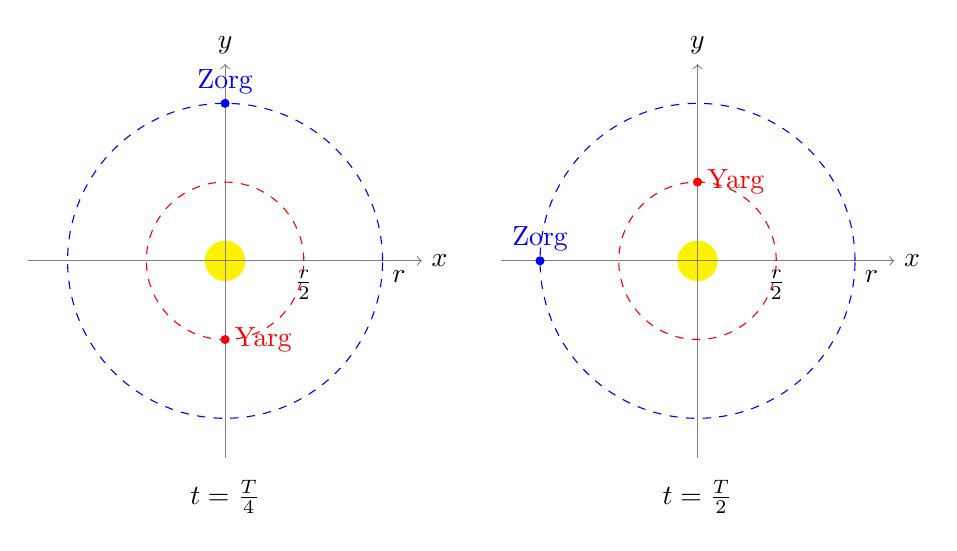
\begin{tikzpicture}[scale = 0.5]
\draw[fill,yellow] (0,0) circle[radius = 0.5];
\draw[gray,->] (-5,0) -- (5,0);
\node[right] at (5,0) {$x$};
\draw[gray,->] (0,-5) -- (0,5);
\node[above] at (0,5) {$y$};

\draw[fill,blue] (0,4) circle[radius=0.1];
\node[above, blue] at (0,4) {Zorg};
\draw[dashed,blue] (0,0) circle[radius=4];

\draw[fill,red] (0,-2) circle[radius=0.1];
\node[right,red] at (0,-2) {Yarg};
\draw[dashed, red] (0,0) circle[radius=2];

\node[below right] at (4,0) {$r$};
\node[below] at (2,0) {$\frac{r}{2}$};

\node at (0,-6) {$t=\frac{T}{4}$};

\draw[fill,yellow] (12,0) circle[radius = 0.5];
\draw[gray,->] (7,0) -- (17,0);
\node[right] at (17,0) {$x$};
\draw[gray,->] (12,-5) -- (12,5);
\node[above] at (12,5) {$y$};

\draw[fill,blue] (8,0) circle[radius=0.1];
\node[above, blue] at (8,0) {Zorg};
\draw[dashed,blue] (12,0) circle[radius=4];

\draw[fill,red] (12,2) circle[radius=0.1];
\node[right,red] at (12,2) {Yarg};
\draw[dashed, red] (12,0) circle[radius=2];

\node[below right] at (16,0) {$r$};
\node[below] at (14,0) {$\frac{r}{2}$};

\node at (12, -6) {$t=\frac{T}{2}$};
\end{tikzpicture}
\end{center}


\begin{center}
\begin{tikzpicture}[scale=0.8]
\draw[fill,yellow] (0,0) circle[radius = 0.5];
\draw[gray,->] (-5,0) -- (5,0);
\node[right] at (5,0) {$x$};
\draw[gray,->] (0,-5) -- (0,5);
\node[above] at (0,5) {$y$};

\draw[fill,blue] (0,-4) circle[radius=0.1];
\node[above, blue] at (0,-4) {Zorg};
\draw[dashed,blue] (0,0) circle[radius=4];

\draw[fill,red] (0,-2) circle[radius=0.1];
\node[right,red] at (0,-2) {Yarg};
\draw[dashed, red] (0,0) circle[radius=2];

\node[below right] at (4,0) {$r$};
\node[below] at (2,0) {$\frac{r}{2}$};

\node at (0,-6) {$t=\frac{3T}{4}$};
\end{tikzpicture}
\end{center}



\clearpage





\textbf{Practice:}

\medskip


Recall the \textbf{compound angle formulae:}
\[\sin(\alpha+\beta)=\sin(\alpha)\cos(\beta)+\cos(\alpha)\sin(\beta)\]
\[\cos(\alpha+\beta)=\cos(\alpha)\cos(\beta)-\sin(\alpha)\sin(\beta)\]
\[\tan(\alpha+\beta)=\frac{\tan(\alpha)+\tan(\beta)}{1-\tan(\alpha)\tan(\beta)}\]


\begin{enumerate}
\item
	\begin{enumerate}
	\item Write down a formula for $\sin(2\theta)$ in terms of $\sin(\theta)$ and $\cos(\theta)$. Hint: $2\theta = \theta + \theta$.
	\item Hence, given that $\sin(12^\circ)\approx 0.208$ and $\cos(12^\circ)\approx 0.978$, find $\sin(24^\circ)$.
	\end{enumerate}
\item \begin{enumerate}
	\item Write down a formula for $\cos(2\theta)$ in terms of $\sin(\theta)$ and $\cos(\theta)$.
	\item Apply the formula $\cos^2(\theta)+\sin^2(\theta)=1$ to eliminate $\sin(\theta)$ from this formula.
	\item Apply the Pythagorean formula again in a different way to your formula from part (a) to eliminate $\cos(\theta)$.
	\end{enumerate}
\item The \textbf{half angle formulae}:
	\begin{enumerate}
	\item Using your answer to question 2(b), express $\cos\left(\theta\right)$ in terms of $\cos(2\theta)$.
	\item Given that $\cos(324^\circ)\approx 0.809$, find $\cos(162^\circ)$.
	\item Using your answer to question 2(c), express $\sin\left(\frac{\theta}{2}\right)$ in terms of $\cos(\theta)$.
	\item Given that $\sin(2.8)\approx 0.335$, find $\sin(1.4)$.
	\end{enumerate}
\item Write down a formula for $\tan(2\theta)$ in terms of $\tan(\theta)$.
Hence, given that $\tan\left(\frac{\pi}{3}\right)=\sqrt{3}$, find $\tan\left(\frac{2\pi}{3}\right)$.
\item \begin{enumerate}
	\item Express $\sin(3\theta)$ in terms of $\sin(\theta)$, $\sin(2\theta)$, $\cos(\theta)$, and $\cos(2\theta)$. Hint: $3\theta=2\theta+\theta$.
	\item Hence express $\sin(3\theta)$ in terms of $\sin(\theta)$ and $\cos(\theta)$ only. Hint: use your answers to questions 1 and 2.
	\item Eliminate $\cos(\theta)$ to obtain an expression for $\sin(3\theta)$ in terms of $\sin(\theta)$ only.
	\end{enumerate}
\item Apply the compound angle formula for cosine to the expression
\[\cos(\alpha+\beta) + \cos(\alpha-\beta).\]
Hence write $\cos(5x)\cos(10x)$ as a sum of two cosines.
\item Apply the compound angle formula for cosine to the expression
\[\cos(\alpha-\beta) - \cos(\alpha+\beta).\]
Hence write $\sin(12\pi t)\sin(2\pi t)$ as a sum of cosines.
\end{enumerate}






\clearpage

\textbf{Theory---Sums of Sinusoids of Equal Frequency:}

\vspace{5mm}

The compound angle formulae split a single sine or cosine into a combination of sines and cosines:
\[\sin(\alpha+\beta) = \sin(\alpha)\cos(\beta)+\cos(\alpha)\sin(\beta),\]
\[\cos(\alpha+\beta) = \cos(\alpha)\cos(\beta)-\sin(\alpha)\sin(\beta).\]
We can use this in reverse to combine sines and cosines \textbf{of the same frequency} into a single sine or cosine.

\vspace{5mm}

Write $3\cos(7\theta)-4\sin(7\theta)$ in the form $R\cos(7\theta+\alpha)$ for some $R$ and $\alpha$.

\vfill

Hence solve $3\cos(7\theta)-4\sin(7\theta)=\frac{1}{\sqrt{2}}$ for $0\leq \theta<\pi$.

\vfill



\clearpage



Here we show the graphs of the functions from the last page:

\begin{center}
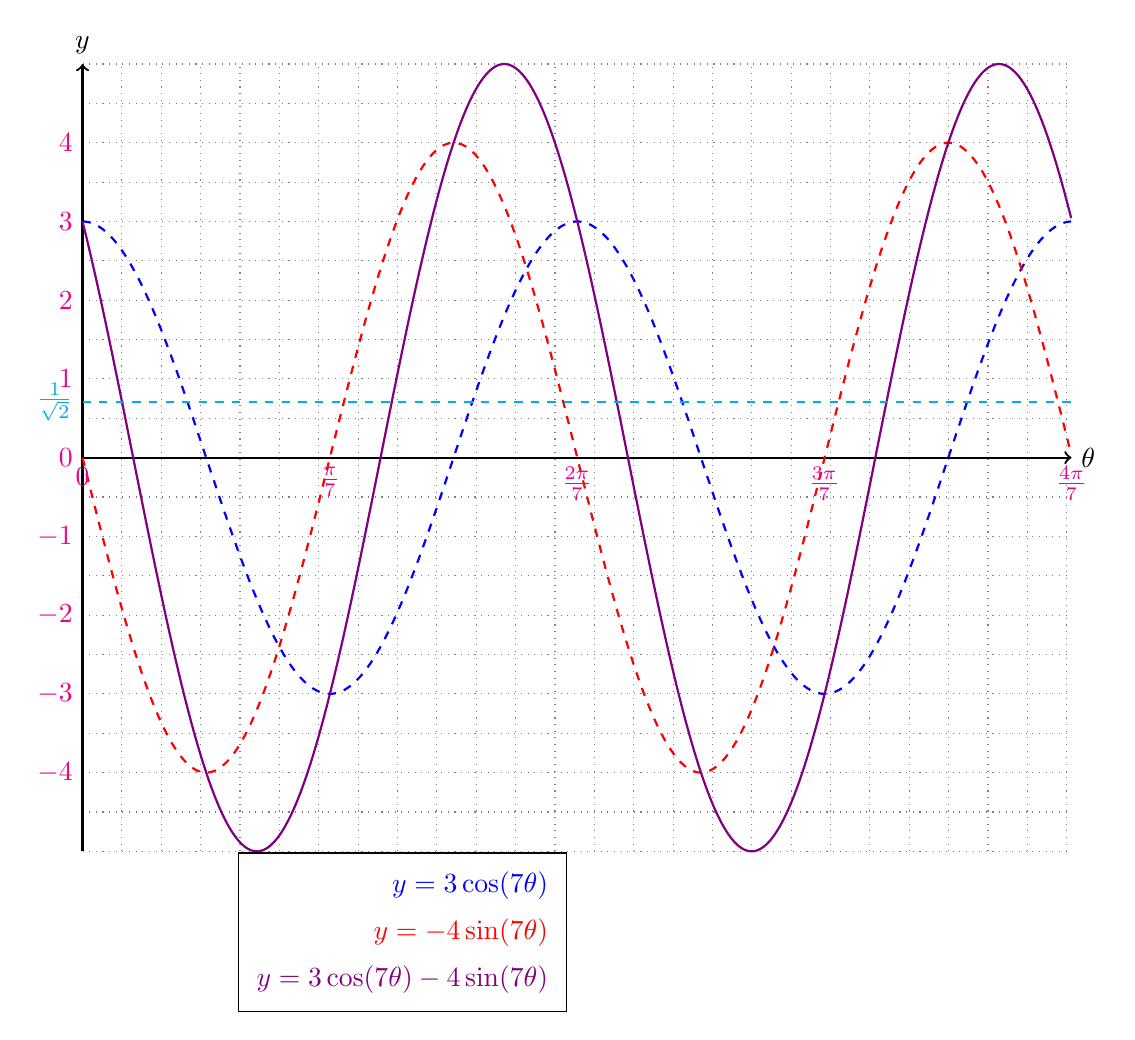
\begin{tikzpicture}
\draw[white] (0,0) -- (13,0);
\draw[step=0.5,gray,thin,dotted] (0,-5) grid (12.56,5);
\draw[thick, ->] (0,-5) -- (0,5);
\node[above] at (0,5) {$y$};
\draw[thick,->] (0,0) -- (12.56,0);
\node[right] at (12.56,0) {$\theta$};

\draw[blue,thick, dashed, domain=0:12.56, samples=300] plot (\x,{3*cos((\x) r)});
\draw[red,thick, dashed, domain=0:12.56, samples=300] plot (\x,{-4*sin((\x) r)});
\draw[violet,thick, domain=0:12.56, samples=300] plot (\x,{3*cos((\x) r) - 4*sin((\x) r)});

\node[magenta,below] at (0,0) {0};
\node[magenta,below] at (3.14,0) {$\frac{\pi}{7}$};
\node[magenta,below] at (6.28,0) {$\frac{2\pi}{7}$};
\node[magenta,below] at (9.42,0) {$\frac{3\pi}{7}$};
\node[magenta,below] at (12.56,0) {$\frac{4\pi}{7}$};


\foreach \i in {-4,-3,-2,-1,0,1,2,3,4}{
	\node[left,magenta] at (0,\i) {$\i$};
	}

	
\draw[cyan,dashed] (0,0.707) -- (12.56,0.707);
\node[cyan,left] at (0,0.707) {$\frac{1}{\sqrt{2}}$};
	
\matrix [draw,below left] at (current bounding box.south) {
	\node [blue] {$y=3\cos(7\theta)$}; \\
	\node [red] {$y=-4\sin(7\theta)$}; \\
	\node[violet] {$y=3\cos(7\theta)-4\sin(7\theta)$};\\
};
\end{tikzpicture}
\end{center}






\clearpage






\textbf{Practice:}

\vspace{5mm}


\begin{enumerate}
\item Express $\sin(3t)-\sqrt{3}\cos(3t)$ in the form $R\sin(3t-\alpha)$.
\item Solve the equation $6\cos(4x)+8\sin(4x) = -0.5$ for $0\leq x<\frac{\pi}{2}$.
\item The voltage of mains electricity varies with time by the function $230\sqrt{2}\sin(100\pi t)$. A drive coil on a so-called ``3-phase'' electric motor receives two alternating voltages, with a time offset between them:
\[A=230\sqrt{2}\sin(100\pi t),\qquad\qquad B=230\sqrt{2}\sin\left(100\pi t+\frac{2\pi}{3}\right).\]
The resulting voltage on the drive coil is $A-B$, the difference between these two voltages. Express the resulting voltage on the drive coil as a single sine function of time; \textit{i.e.}, write $A-B$ in the form $R\sin(100\pi t+\alpha)$. Hence suggest why for high-power applications 3-phase motors are used instead of single phase motors (with just one mains voltage applied).
\item Sound is a pressure wave in the air; for a single pure note at frequency $f$ and amplitude $A$, the pressure $P_1$ at a point in the air varies with time according to $P_1=A\sin(2\pi f t)$. When two sounds are played, with pressure waves $P_1$ and $P_2$, the overall effect on air pressure is $P_1+P_2$.

Suppose an additional sound is played, with $P_2=A\sin\left((2\pi+1) ft\right)$. The overall result of these two pressure waves is that the total air pressure is $P_{\mathrm{total}}=P_1+P_2$. Apply the compound angle formula for sine to $P_2$ and hence find $P_\mathrm{total}$. Describe the sound which results when both these sounds are played together, and hence suggest how noise-cancelling headphones work.
\end{enumerate}



\clearpage


\textbf{Key Points to Remember:}

\begin{enumerate}
\item The \textbf{compound angle formulae} for sine and cosine are:
	\[\cos(\alpha+\beta)=\cos(\alpha)\cos(\beta)-\sin(\alpha)\sin(\beta)\]
	\[\sin(\alpha+\beta)=\sin(\alpha)\cos(\beta)+\cos(\alpha)\sin(\beta)\]
\item We can decompose the product of two sines or of two cosines:
	\[\cos(\alpha)\cos(\beta)=\frac{1}{2}\left(\cos(\alpha+\beta)+\cos(\alpha-\beta)\right)\]
	\[\sin(\alpha)\sin(\beta) = \frac{1}{2}\left(\cos(\alpha-\beta)-\cos(\alpha+\beta)\right)\]
\item We can express a sum of sinusoids \textbf{of the same frequency} (and any phase and amplitude) as a single sinusoid:
	\[A\sin(\omega t+\phi)+B\cos(\omega t+\psi) = R\sin(\omega t+\alpha) \mbox{ or } S\cos(\omega t+\beta)\]
	where	$R$ and $\alpha$ (or $S$ and $\beta$) are found by expanding the right-hand side with a compound angle formula and comparing coefficients of $\sin$ and of $\cos$.
\item The sum of sinusoids \textbf{of the same frequency} is a sinusoid. The product of sinusoids, or the sum of sinusoids of different frequencies, is a more complicated waveform.
\end{enumerate}




\end{document}